\subsection{Mutierende globale Problemmenge}
\begin{figure}[H]
  \centering
  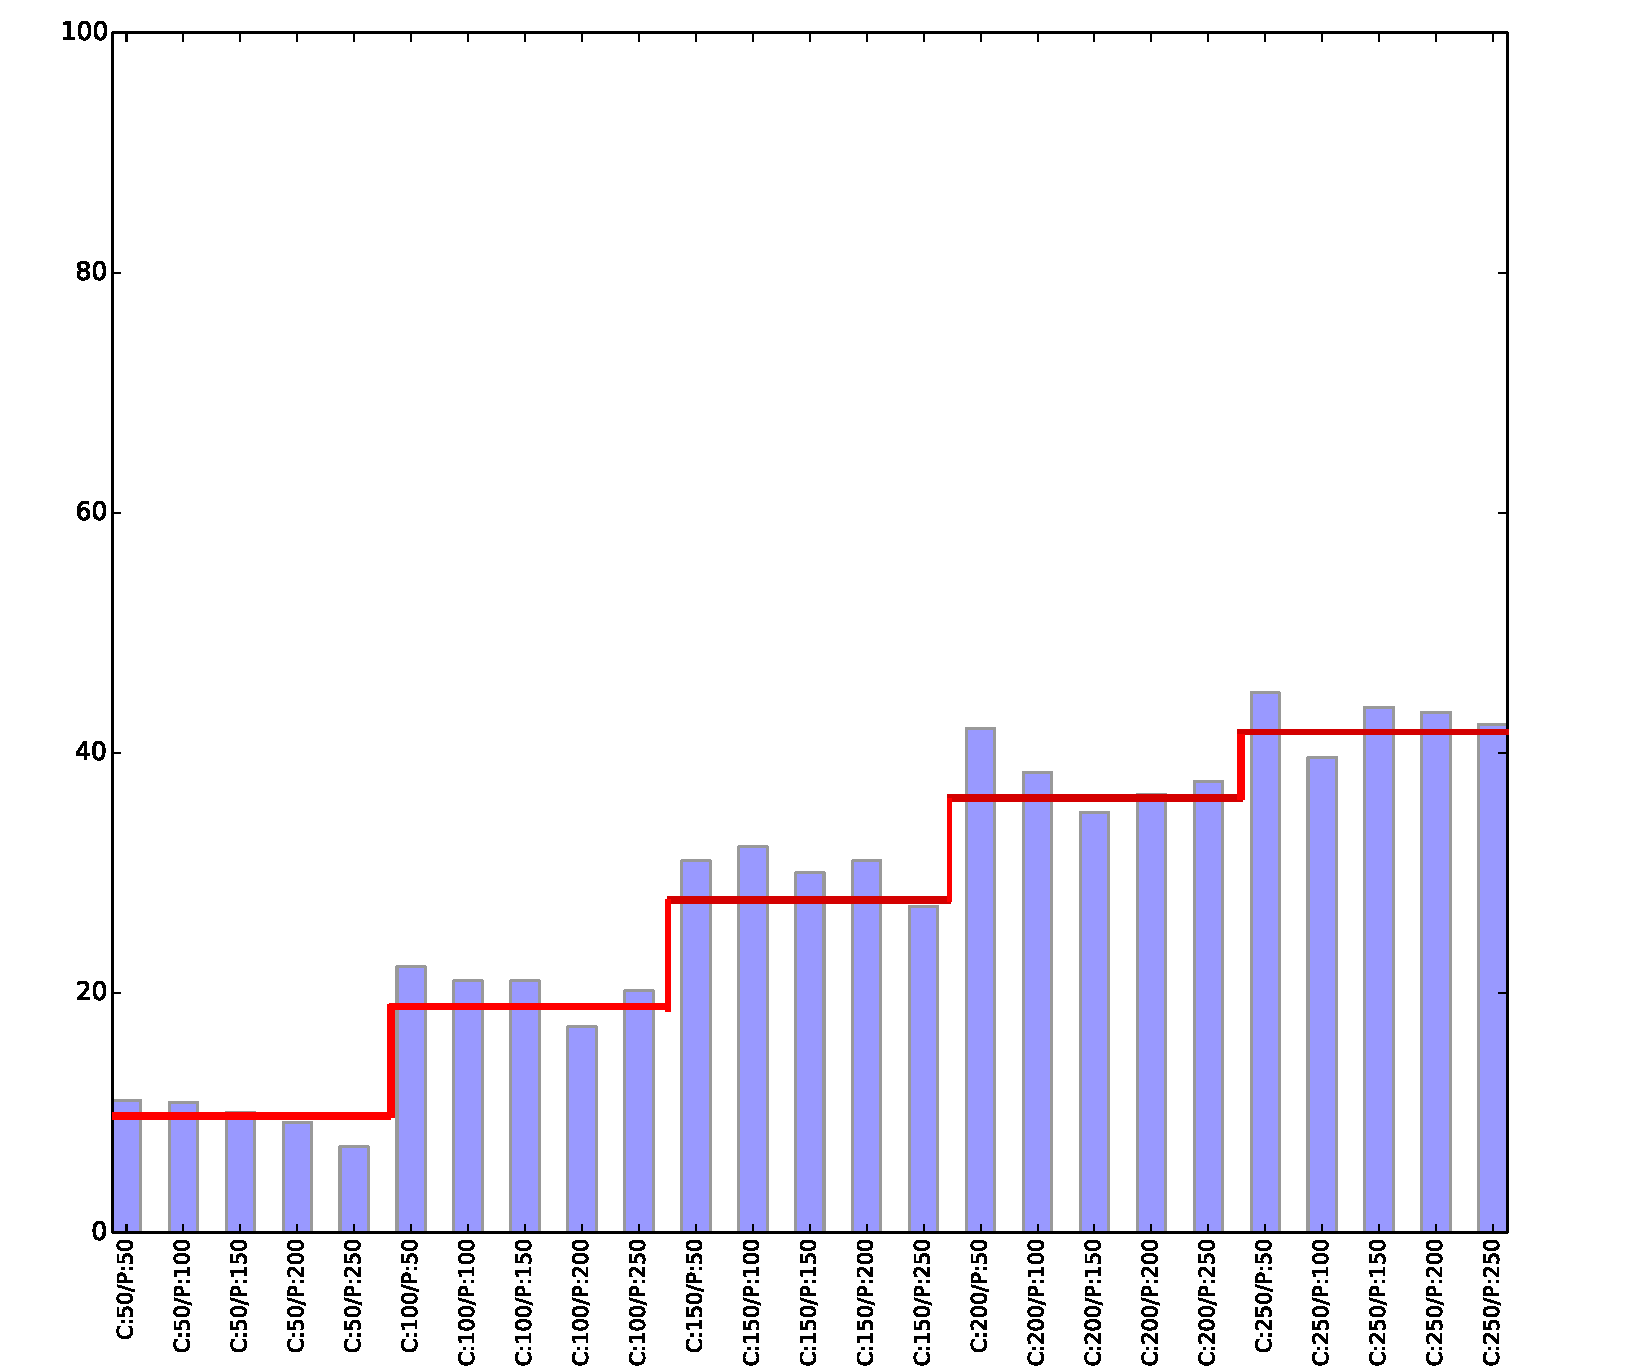
\includegraphics[width=0.8\textwidth]{images/E_G_abab_solved.pdf}
  \caption[ABAB Problem - Globale Mutierende Problemmenge]{ABAB Problem - Globale Mutierende Problemmenge}
  \label{fig:e_g_abab}
\end{figure}
Die untersuchten evolutionären Algorithmen mit einer globalen mutierenden Problemmenge haben im Gegensatz zum Ansatz mit den Festen globalen Problemmengen ein sehr spezielles Skalierungsverhalten im Bezug auf die grösse der Problemmenge an den Tag gelegt.

Die Eingabeparameter für die Abbildung \ref{fig:e_g_abab} waren:
\begin{itemize}
	\item Grösse der Problemmenge: 50, 100, 150, 200, 250
	\item Anzahl der Lösungskandidaten: 50, 100, 150, 200, 250
\end{itemize}

In Abbildung \ref{fig:e_g_abab} ist ersichtlich wie sich ein \flqq teppenförmiges\frqq Muster abzeichnet. Daraus könnte man schliessen, dass der Algorithmus unabhängig von der Problemmengengrösse eigentlich immer gleich oft konvergiert. Um diese These zu überprüfen wurde auch mit diesem Algorithmus ein Test bei konstanter Anzahl Lösungskandidaten durchgeführt. Als Problem der Wahl wurde hier aus Gründen der Vergleichbarkeit wieder das durch fünf Teilbar Problem gewählt.
\begin{figure}[H]
  \centering
  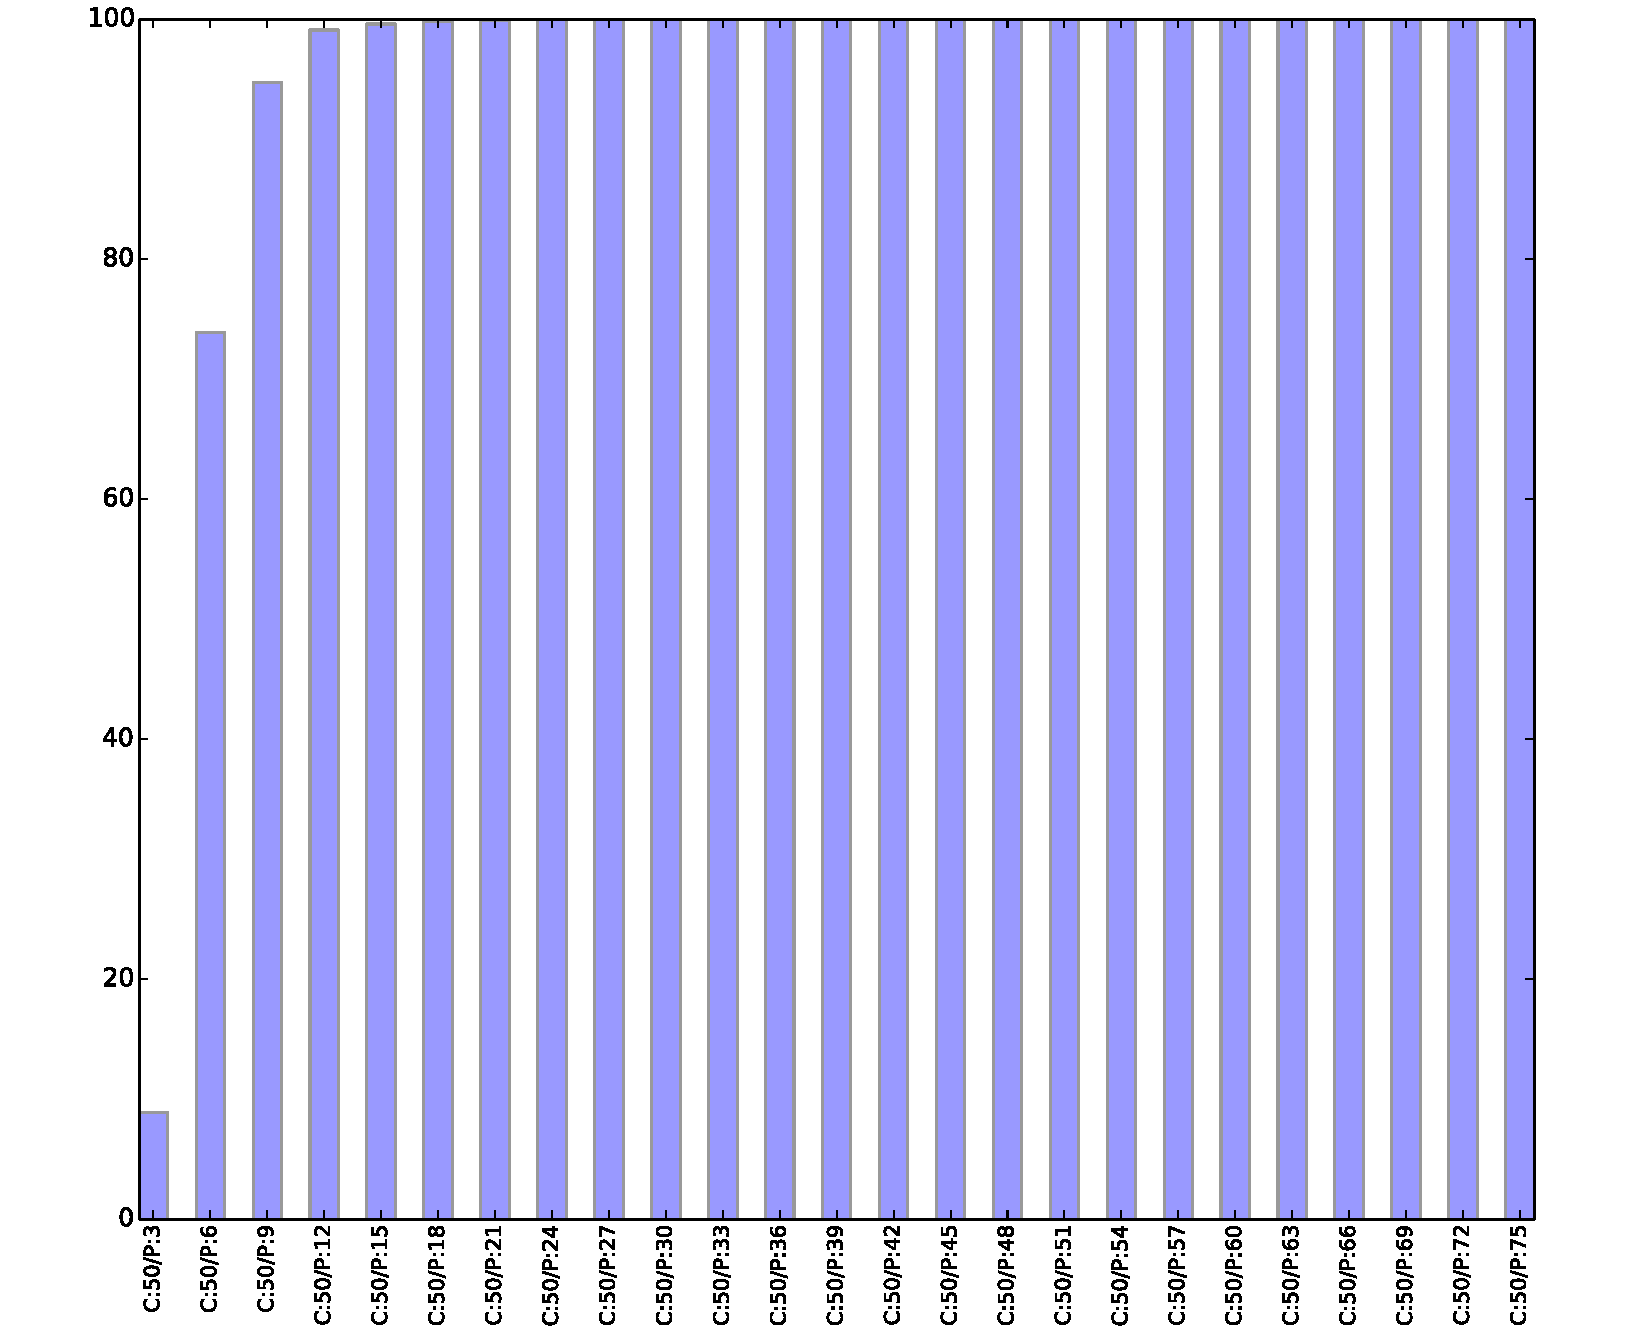
\includegraphics[width=0.78\textwidth]{images/E_G_PS_div5PS_solved.pdf}
  \caption[GM Algorithmus - Skalierung mit Problemmengengrösse]{GM Algorithmus - Skalierung mit Problemmengengrösse}
  \label{fig:e_g_ps_div5}
\end{figure}
\pagebreak
Die Eingabeparameter für die Abbildung \ref{fig:e_g_ps_div5} waren:
\begin{itemize}
	\item Grösse der Problemmenge: 3, 6, 9, 12, ..., 72, 75
	\item Anzahl der Lösungskandidaten: 50
\end{itemize}

Bei diesem Versuch (Abbildung \ref{fig:e_g_ps_div5}) sieht man, dass auch dieser Algorithmus mit sehr kleinen Problemmengen ($3$ oder $6$ Probleme) mühe hat. Jedoch konvergiert er bereits ab circa 10 Problemen in jedem Fall. Das heisst, sobald eine kritische Problemmengengrösse erreicht wurde, hat ein weiteres erhöhen dieser keinen Einfluss mehr auf das Konvergenzverhalten dieses Algorithmus.

Das bedeutet, dass diese Art von evoultionären Algorithmen primär mit der Anzahl Lösungskandidaten skalieren. Welches die Optimale Problemmengengrösse für ein konkretes Problem ist, muss individuell geprüft werden. Für unser Problem der durch fünf teilbaren Binärzahlen konvergiert zum Beispiel bereits ab 20 Problemen sehr zuverlässig.

Um zu prüfen wie das Konvergenzverhalten in Abhängigkeit der Anzahl Lösungskandidaten ist, wurde auch hierzu entsprechende Daten gesammelt.
\begin{figure}[H]
  \centering
  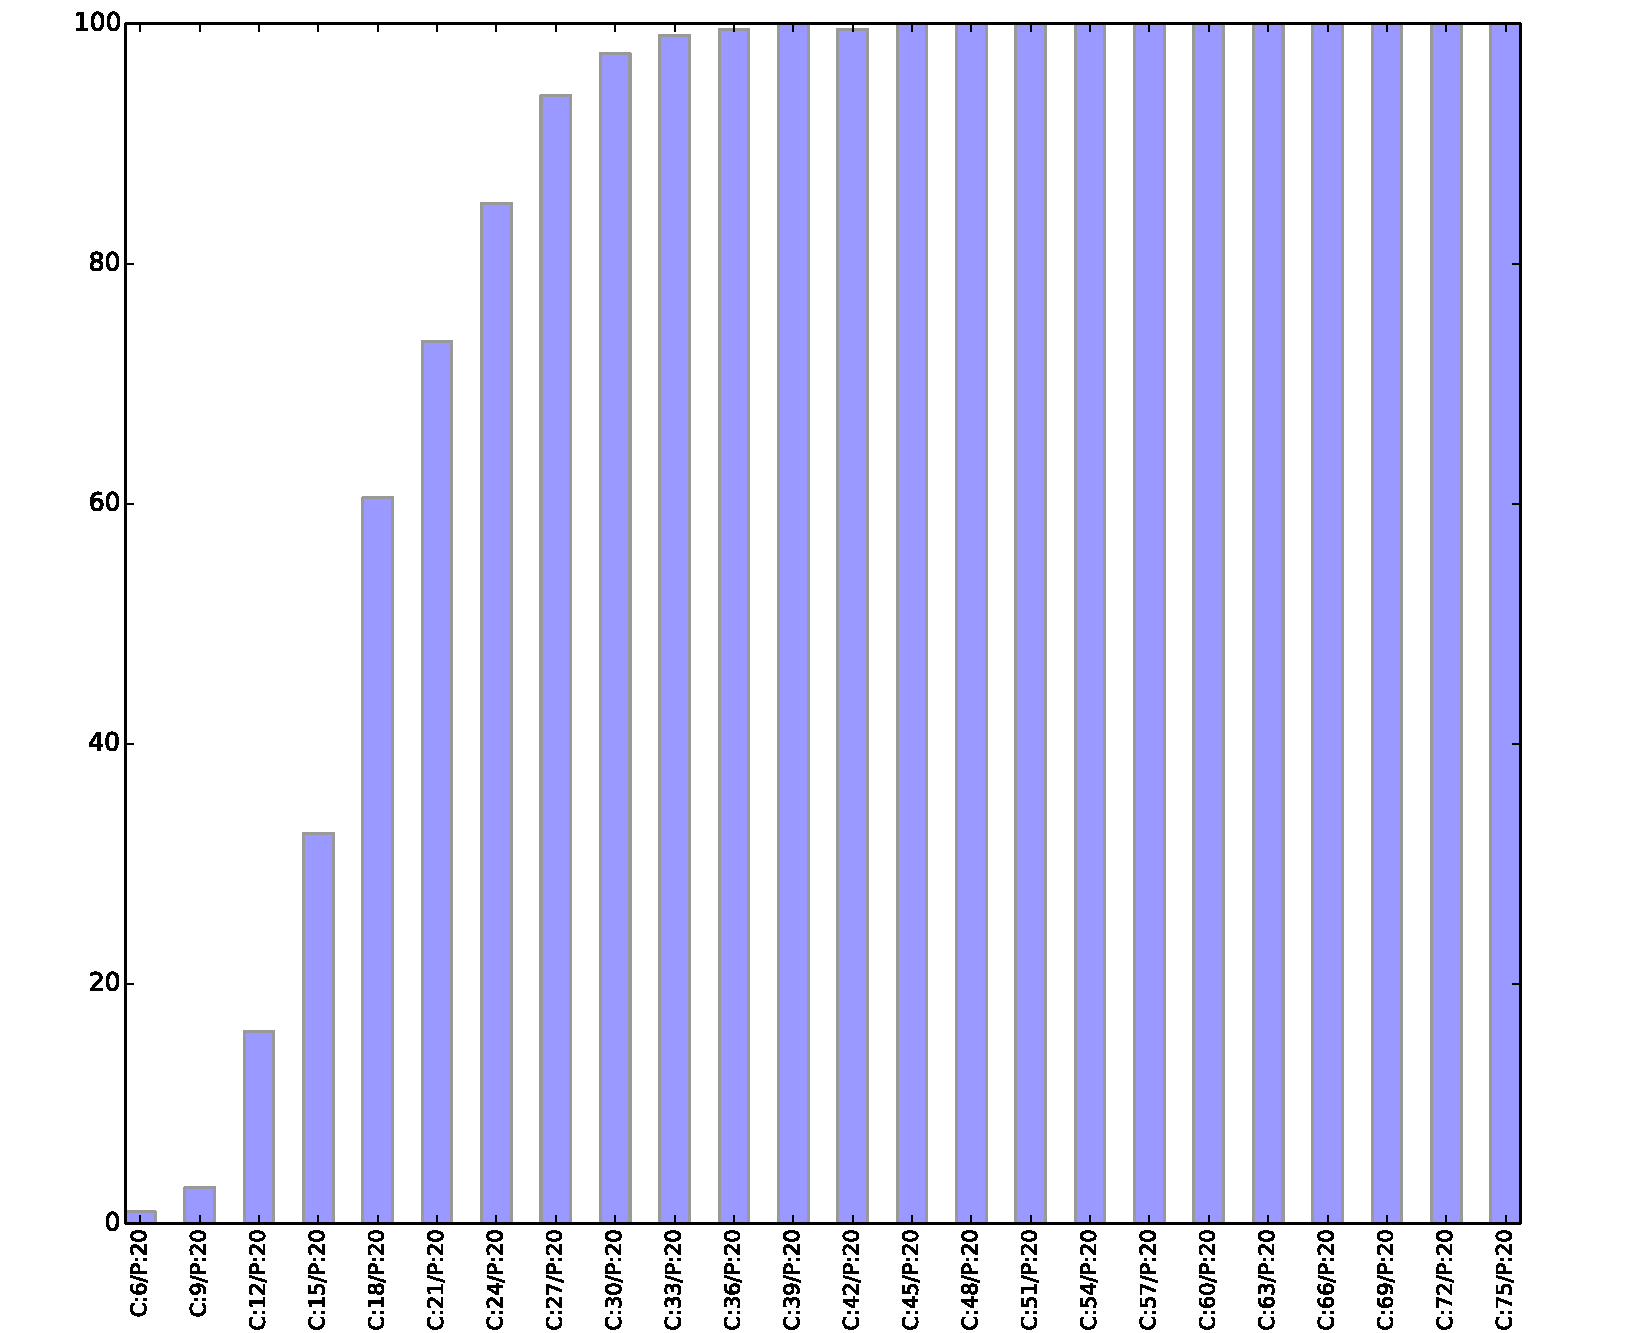
\includegraphics[width=0.78\textwidth]{images/E_G_CS_div5CS_solved.pdf}
  \caption[GM Algorithmus - Skalierung mit Anzahl Lösungskandidaten]{GM Algorithmus - Skalierung mit Anzahl Lösungskandidaten}
  \label{fig:e_g_cs_div5}
\end{figure}
Die Eingabeparameter für die Abbildung \ref{fig:e_g_cs_div5} waren:
\begin{itemize}
	\item Grösse der Problemmenge: 20
	\item Anzahl der Lösungskandidaten: 3, 6, 9, 12, ..., 72, 75
\end{itemize}

In dieser Abbildung sieht man erneut, dass zu wenige Lösungskandidaten ein Problem sind. Der steile Anstieg der Konvergenzrate und das Abflachen (in diesem Fall sogar erreichen der 100\% Marke) ist vergleichbar mit dem Verhalten des Algorithmus mit konstanter Problemmenge.